\documentclass{beamer}
\usepackage{ctex, hyperref}
\usepackage[T1]{fontenc}

% other packages
\usepackage{latexsym,amsmath,xcolor,multicol,booktabs,calligra}
\usepackage{graphicx,pstricks,listings,stackengine}
\usepackage{textcomp}

\author{谭诗弘，黄育民，曹洪珲}
\title{智能系统设计实践}
\subtitle{六足机器人避障控制 结题汇报}
\institute{武汉大学电子信息学院}
\date{2025年11月3日}
\usepackage{whu}

% defs
\def\cmd#1{\texttt{\color{red}\footnotesize $\backslash$#1}}
\def\env#1{\texttt{\color{blue}\footnotesize #1}}
\definecolor{deepblue}{rgb}{0,0,0.5}
\definecolor{deepred}{rgb}{0.6,0,0}
\definecolor{deepgreen}{rgb}{0,0.5,0}
\definecolor{halfgray}{gray}{0.55}

\lstset{
    basicstyle=\ttfamily\small,
    keywordstyle=\bfseries\color{deepblue},
    emphstyle=\ttfamily\color{deepred},    % Custom highlighting style
    stringstyle=\color{deepgreen},
    numbers=left,
    numberstyle=\small\color{halfgray},
    rulesepcolor=\color{red!20!green!20!blue!20},
    frame=shadowbox,
}


\begin{document}

\kaishu
\begin{frame}
    \titlepage
    \begin{figure}[htpb]
        \begin{center}
            
\includegraphics[width=0.2\linewidth]{pic/whulogo.png}
        \end{center}
    \end{figure}
\end{frame}

% \begin{frame}
%     \tableofcontents[sectionstyle=show,subsectionstyle=show/shaded/hide,subsubsectionstyle=show/shaded/hide]
% \end{frame}


\section{课题背景}

% \begin{frame}{课题背景}
%     \begin{itemize}[<+-| alert@+>] % 当然，除了alert，手动在里面插 \pause 也行
%         \item 大家都会\LaTeX{}，好多学校都有自己的Beamer主题
%         \item 中文支持请选择 Xe\LaTeX{} 编译选项
%         \item 原 THU Beamer Github项目地址位于 \url{https://github.com/tuna/THU-Beamer-Theme}
%         \item 本魔改 GitHub项目地址位于 \url{https://github.com/Xinchen-Fan/WHU-Beamer-Theme}，如果有bug或者feature request可以去里面提issue
%     \end{itemize}
% \end{frame}

\begin{frame}{六足机器人业界现状}
    近年来，随着人工智能、机器人技术与自动控制理论的发展，仿生机器人逐渐成为研究热点。
    六足机器人凭借以下优势：
    \begin{itemize}
        \item 结构稳定性高
        \item 步态灵活多样
        \item 适应复杂地形能力强
    \end{itemize}

    在灾害救援、地质勘探、军事侦察等领域展现出广阔应用前景。
    与轮式或履带式机器人相比，六足机器人能够在崎岖不平的地形环境下保持稳定行走，
    这为其在野外环境中的任务执行提供了独特优势。

    % 插入三张图片（并列展示）
    \begin{figure}[htpb]
        \centering
        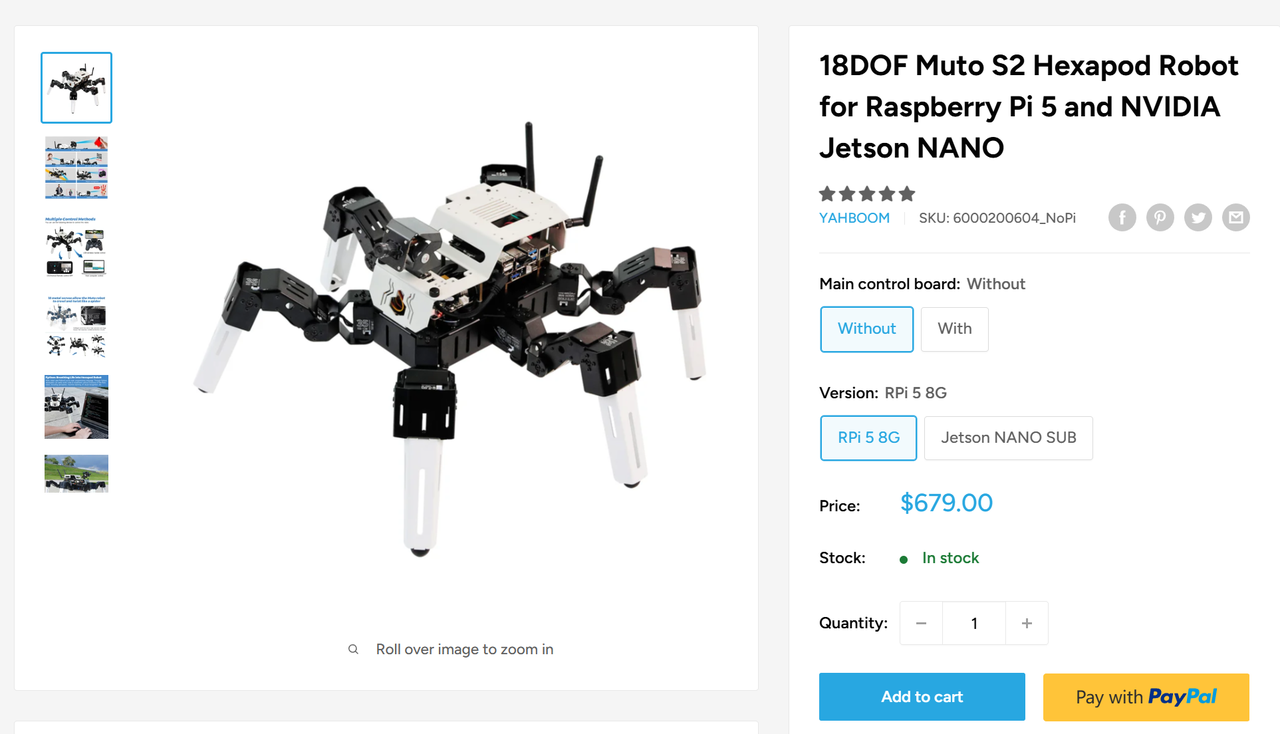
\includegraphics[width=0.3\linewidth]{pic/muto s2.PNG}
        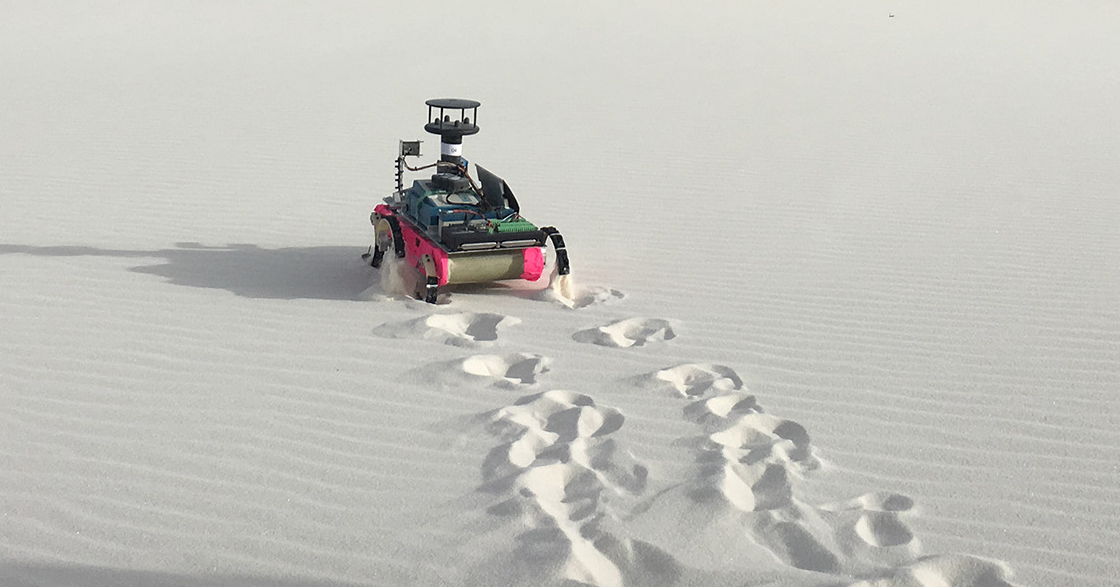
\includegraphics[width=0.3\linewidth]{pic/沙漠六足机器人.png}
        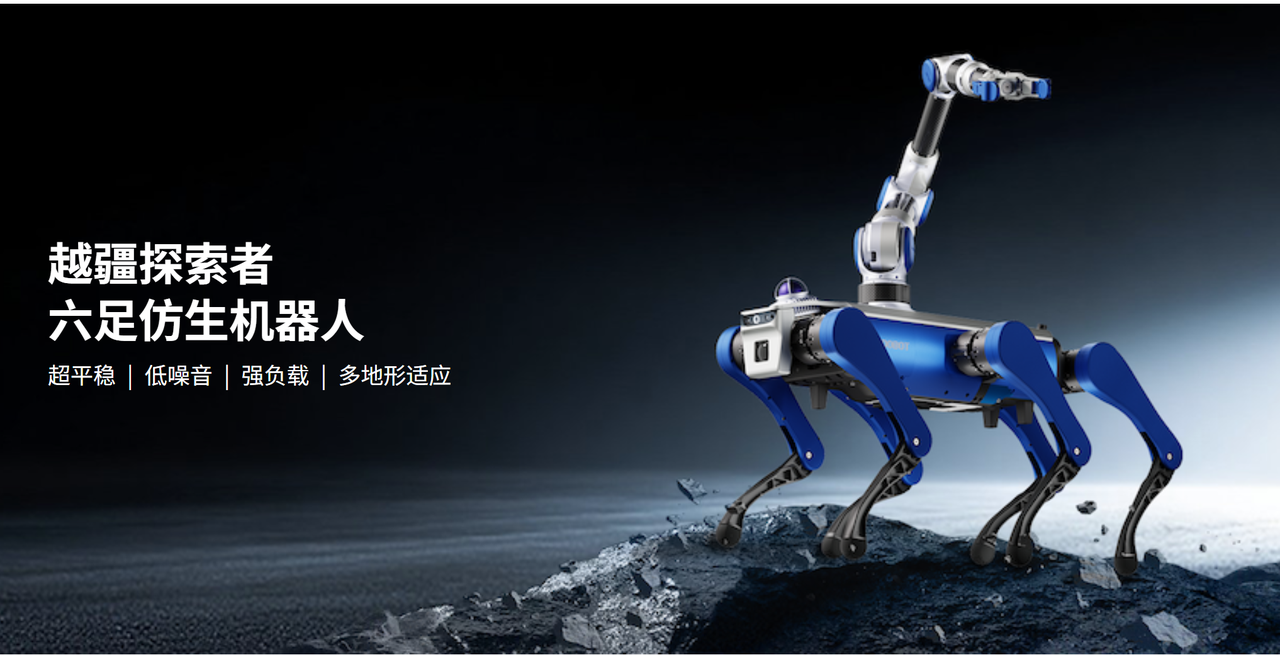
\includegraphics[width=0.3\linewidth]{pic/六足带机械臂狗.png}
    \end{figure}
\end{frame}

\begin{frame}{六足机器人避障的难点与研究动机}
    六足机器人在复杂环境下的自主避障，面临以下挑战：
    \begin{itemize}
        \item \textbf{姿态控制复杂}：六足机器人具有多个自由度，
              在避障过程中需要同时兼顾 \textbf{步态稳定性、能耗优化和绕障效率}。
        \item \textbf{视觉与控制耦合困难}：视觉传感器获取的环境信息
              存在 \textbf{延迟、噪声和不确定性}，如何与实时步态调整协调仍是难题。
        \item \textbf{环境动态性强}：障碍物的形态与分布复杂，
              导致传统静态路径规划方法难以满足实时避障需求。
    \end{itemize}

    \vspace{0.3cm}
    \textbf{研究动机：}  
    本课题旨在探索 \textbf{六足机器人多足步态控制并实现避障}的方法，
    提升其在复杂环境下的避障能力与自主性。
\end{frame}

\section{前期研究}

\begin{frame}{六足机器人组装测试}
    \begin{figure}[htpb]
        \centering
        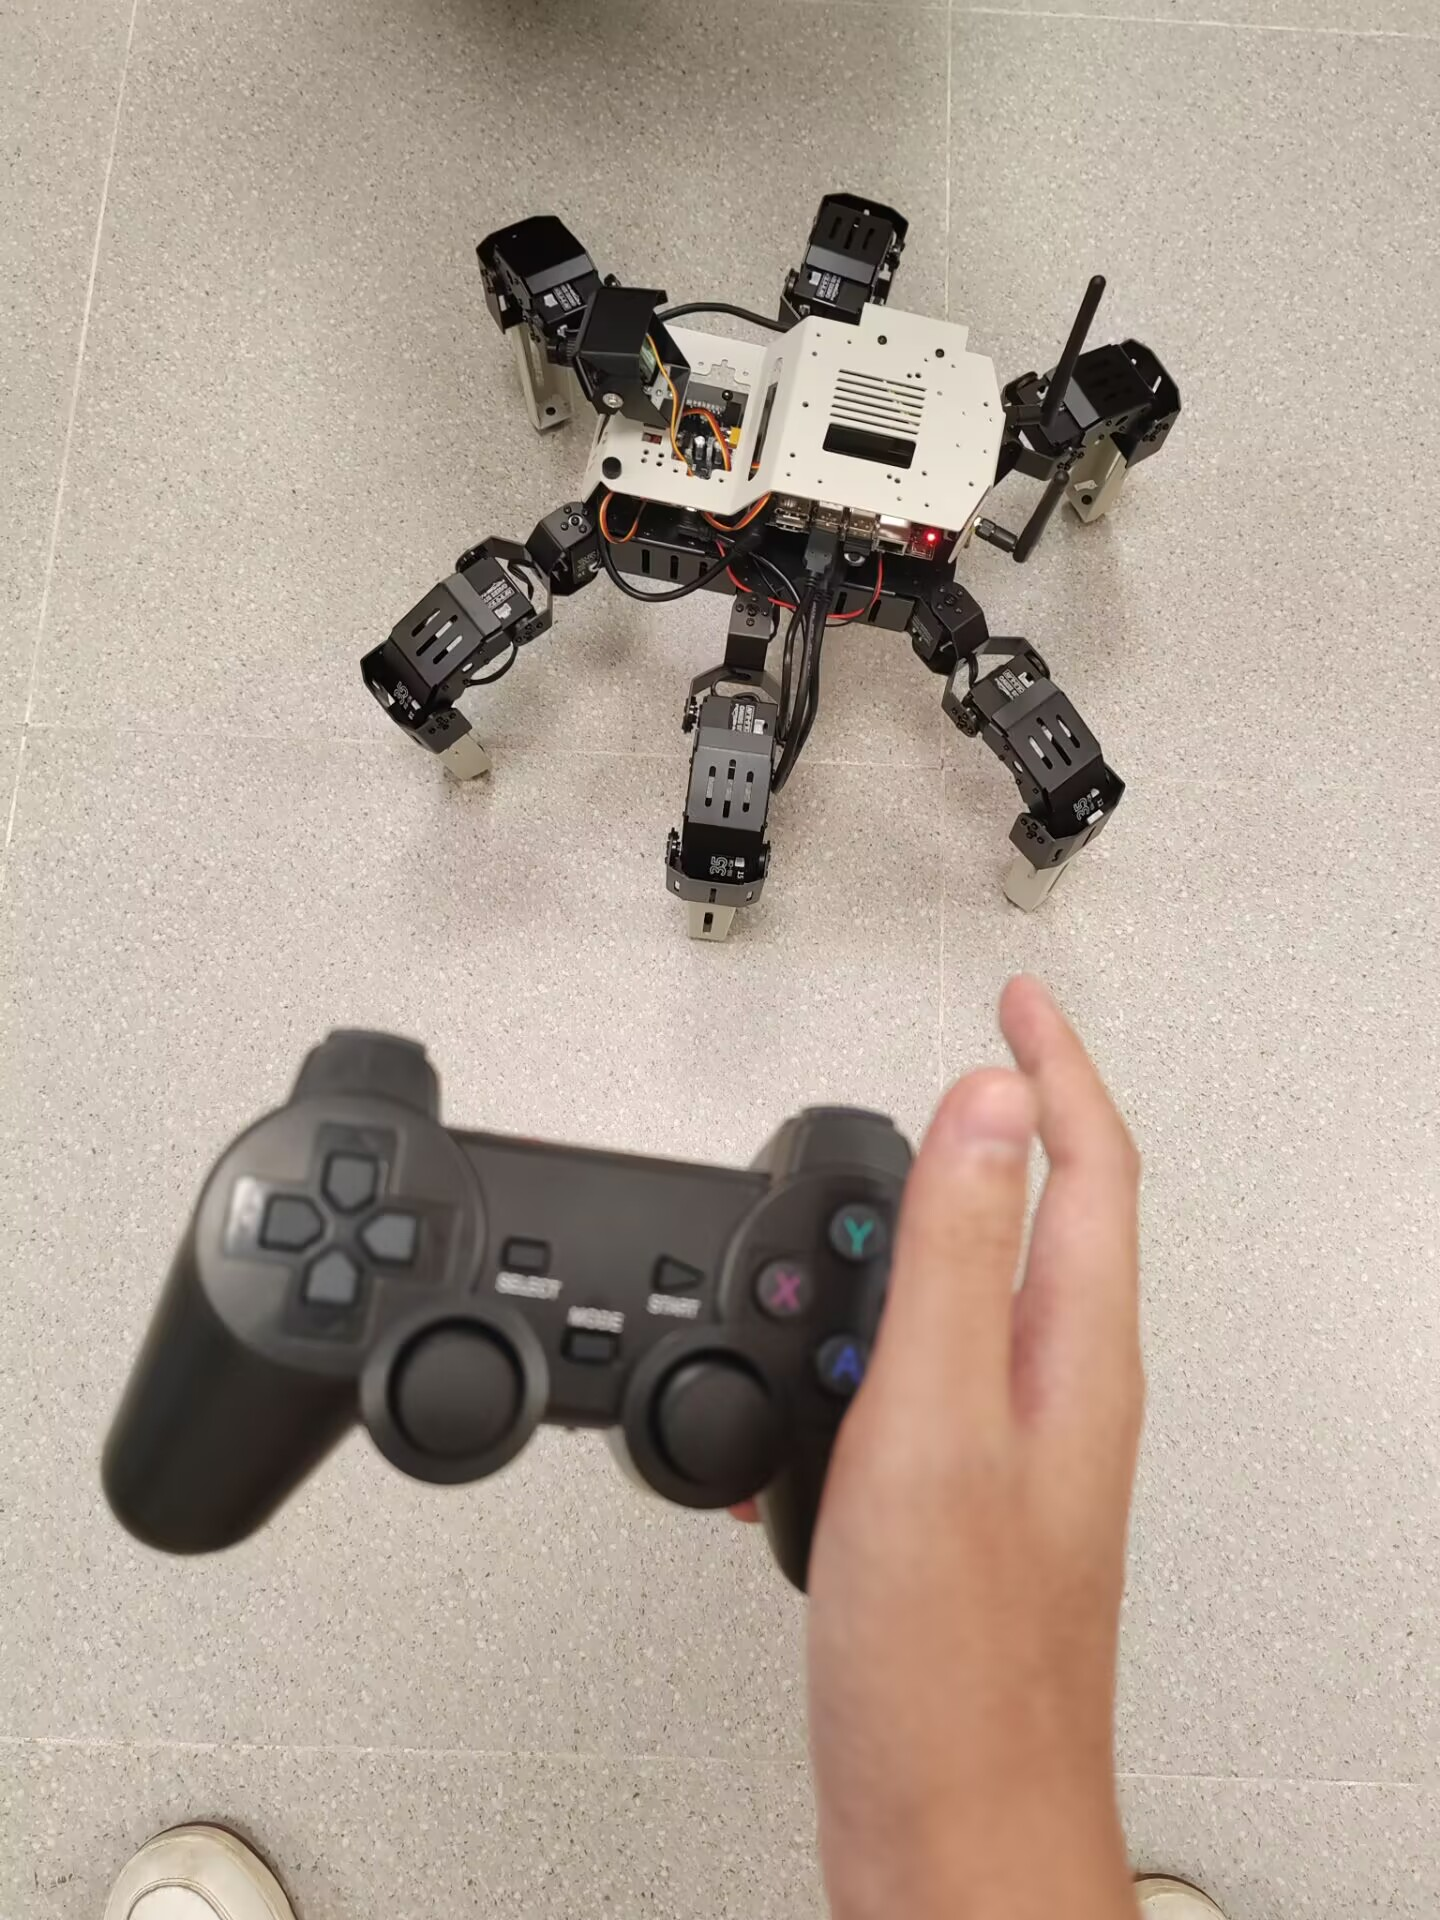
\includegraphics[width=0.49\linewidth]{pic/hex.jpg}
        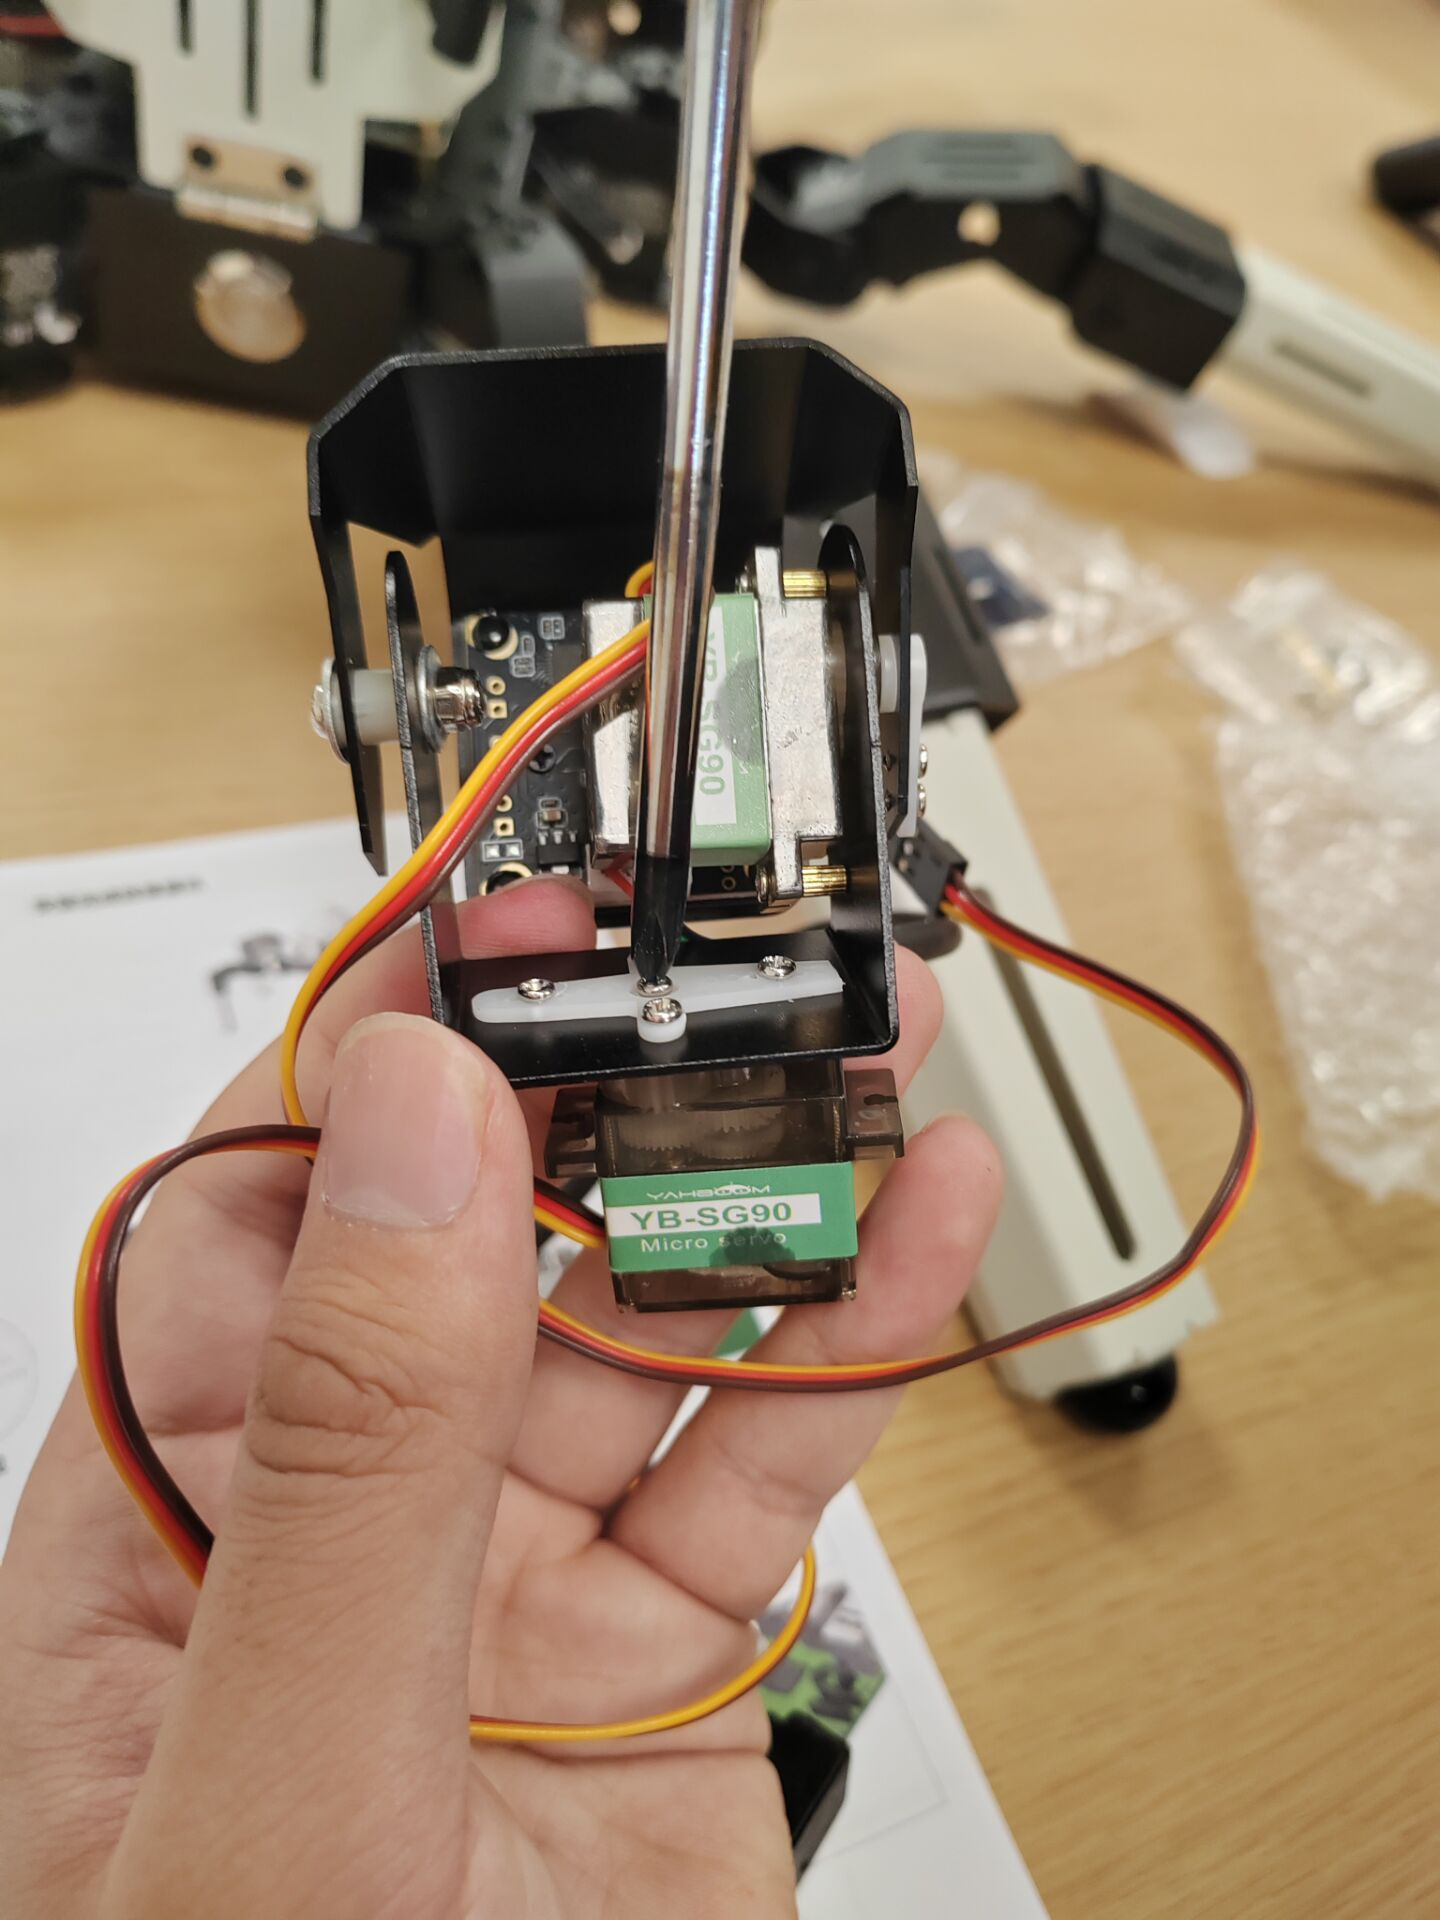
\includegraphics[width=0.49\linewidth]{pic/constr.jpg}
    \end{figure}
\end{frame}

\begin{frame}{六足机器人硬件架构}
    \begin{figure}[htpb]
        \centering
        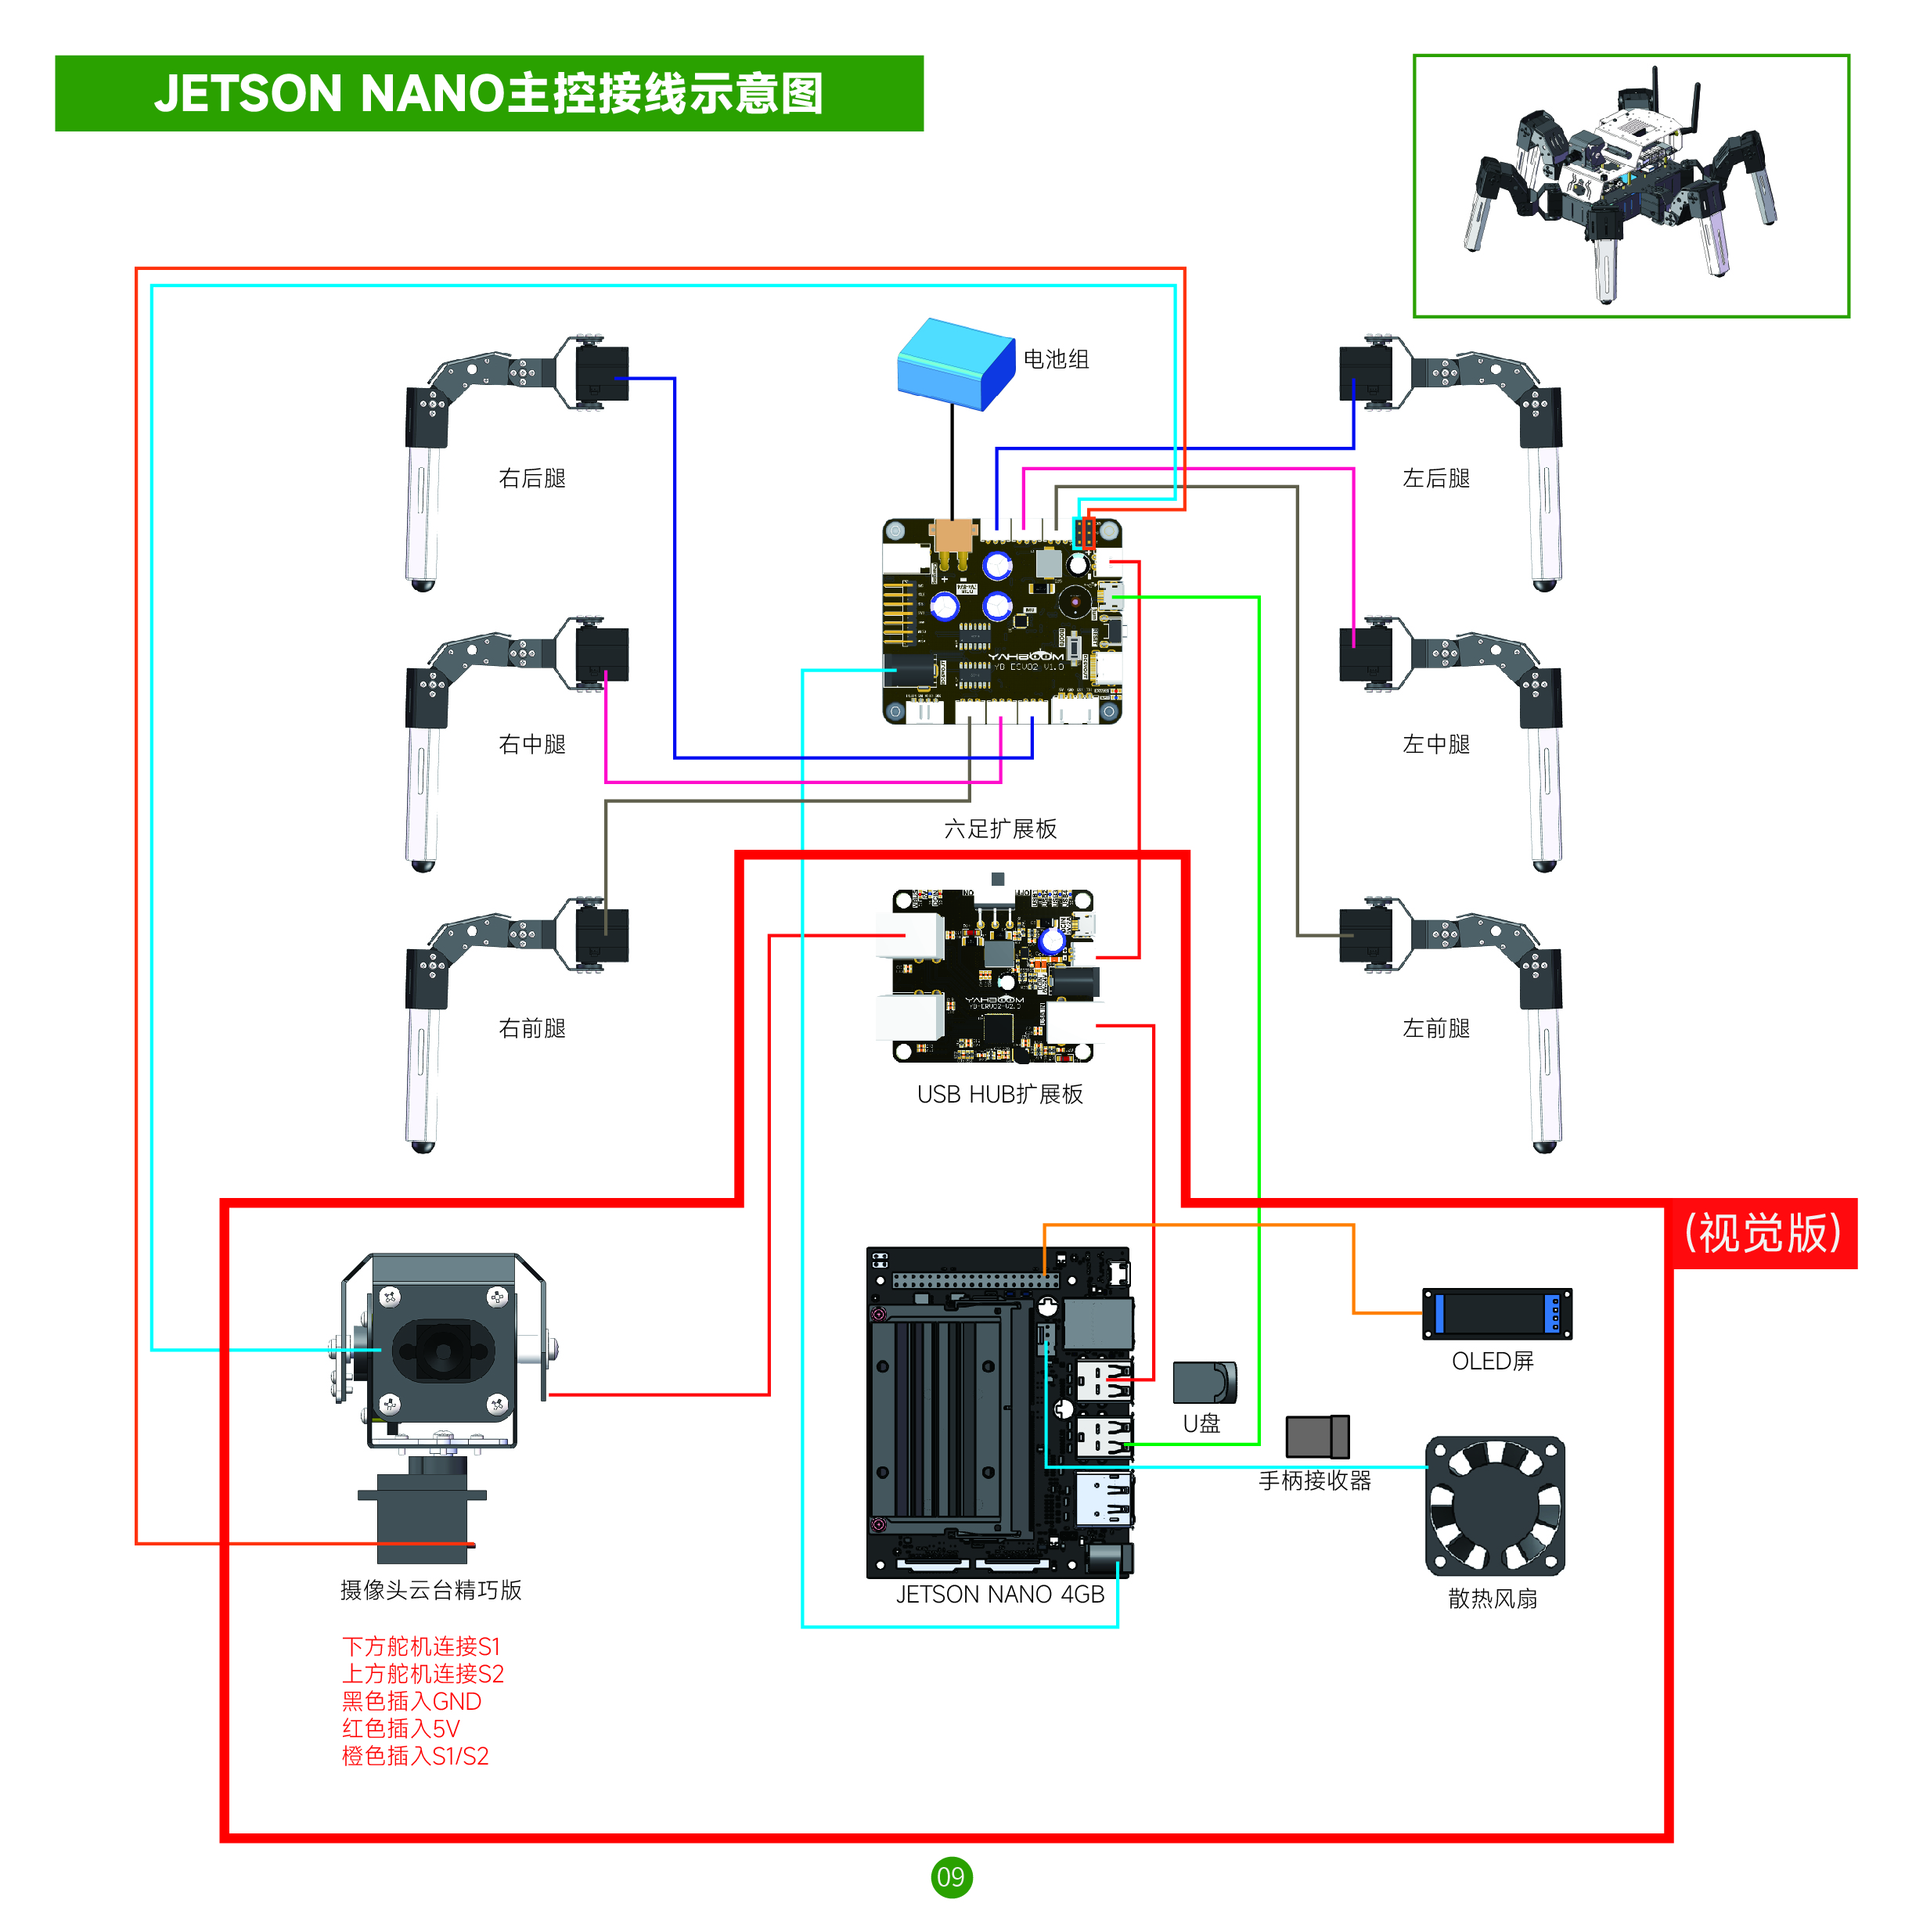
\includegraphics[width=0.6\linewidth]{pic/arch.jpg}
    \end{figure}
\end{frame}

\begin{frame}{六足机器人硬件架构}
    \begin{itemize}
        \item 顶层（Jetson Nano）：
        \\ 负责路径规划、目标识别、避障算法、通信等功能，通过串口/总线将指令下发给STM32扩展板。Jetson Nano采用带桌面的Ubuntu作为操作系统。
        \item 底层（STM32控制板）：
        \\ 负责PWM舵机驱动、步态切换、姿态保持、传感器数据读取等，通过预设的步态算法执行任务。
        \item 单腿硬件：
        \\ 每只腿包含3个舵机，分别是：肩关节（控制腿向前/后/侧方向摆动，决定运动方向（前进、转向、横移）），大腿关节（控制大腿的抬起和放下）和膝关节（控制小腿弯曲/伸直，影响步幅长度和对地形的适应性。）。
    \end{itemize}
\end{frame}

\begin{frame}{六足机器人软件架构}
    \begin{itemize}
        \item 人机输入层（操作者）
        \\ 输入设备：手柄 / 手机APP / 键盘 / 上位机 GUI（带摄像头流/深度视图）
        \item 上位控制层（Jetson Nano）
        \\ 接收人控指令、实时显示视频、将高层命令转为步态/动作模板 + 参数、发送到 STM32。使用Python/ROS 节点（推荐 ROS 或 socket 通信）。
        \item 步态规划与变换层（Jetson Nano或STM32）
        \\ 将“动作命令（如前进、左移、抬右前腿）”转为每条腿的期望足端轨迹（时序/位置/速度）。
        \item 逆运动学与舵机控制层（STM32）
        \\ 把足端轨迹转为 18 个舵机角度，通过 PWM/串口控制舵机；做低级 PID 或 P 控制。
    \end{itemize}
\end{frame}

\section{基础控制方案研究}

\begin{frame}{主要控制文件概览}
    \textbf{共 11 个核心模块：}
    \begin{enumerate}
        \item base.py：基础坐标类与腿尖坐标系
        \item config.py：配置参数与预定义步态轨迹
        \item hexapod.py：六足机器人主控制类
        \item kinematicLib.py：运动学核心（逆运动学、轨迹生成、坐标变换）
        \item leg.py：单腿控制类，负责逆运动学与舵机控制
        \item movement\_paths.py：预定义步态轨迹数据库
        \item movement.py：高层动作控制器（模式切换、轨迹调度）
        \item movement\_table.py：静态动作路径表
        \item MutoLib.py：机器人与上位机通信接口
        \item pathPlanning.py：路径规划模块
        \item servo.py：舵机控制模块
    \end{enumerate}
\end{frame}

% % ---------------------------
% \begin{frame}{模块分层结构图（详细版）}
% \centering
% \scalebox{0.75}{
% \begin{tikzpicture}[node distance=0.6cm, every node/.style={draw, rounded corners, align=center, font=\scriptsize, minimum width=2.8cm, minimum height=0.6cm}]
% % 基础层
% \node (base) {基础层 \\ base.py};

% % 配置层
% \node (config) [below=of base] {配置层 \\ config.py};

% % 单腿控制层
% \node (leg) [below=of config] {单腿控制层 \\ leg.py};

% % 运动学与路径层
% \node (kinematic) [below=of leg, xshift=-2.8cm] {kinematicLib.py};
% \node (mvtpaths) [below=of leg] {movement\_paths.py};
% \node (mvttable) [below=of leg, xshift=2.8cm] {movement\_table.py};

% % 动作调度层
% \node (movement) [below=2.5cm of mvtpaths] {动作调度层 \\ movement.py};

% % 整体协调层
% \node (hexapod) [below=of movement] {整体协调层 \\ hexapod.py};

% % 通信层
% \node (muto) [below=of hexapod, xshift=-3.5cm] {通信层 \\ MutoLib.py};

% % 路径规划层
% \node (path) [below=of hexapod, xshift=3.5cm] {路径规划层 \\ pathPlanning.py};

% % 执行层
% \node (servo) [below=2.5cm of hexapod] {执行层 \\ servo.py};

% % Arrows
% \draw[->] (base) -- (config);
% \draw[->] (config) -- (leg);
% \draw[->] (leg) -- (kinematic);
% \draw[->] (leg) -- (mvtpaths);
% \draw[->] (leg) -- (mvttable);
% \draw[->] (kinematic) -- (movement);
% \draw[->] (mvtpaths) -- (movement);
% \draw[->] (mvttable) -- (movement);
% \draw[->] (movement) -- (hexapod);
% \draw[->] (hexapod) -- (servo);O 
% \draw[->] (hexapod) -- (muto);
% \draw[->] (hexapod) -- (path);

% \end{tikzpicture}
% }
% \end{frame}

\begin{frame}{控制流程图}
    \begin{figure}[htpb]
        \centering
        
\includegraphics[width=0.49\linewidth]{pic/soft.png}
    \end{figure}
\end{frame}

\begin{frame}{控制流程总结}
    \begin{enumerate}
        \item 用户输入（例如hexapod.move(10,0,0) $\rightarrow$ 前进10cm）。
        \item movement.py 根据输入调用movement\_table / pathPlanning 生成完整轨迹点。
        \item hexapod.py 轮询调用movement.next() $\rightarrow$ 取出6 条腿的坐标。
        \item leg.py 将目标点$\rightarrow$ 逆运动学角度。
        \item servo.py 把角度$\rightarrow$ 舵机指令。
        \item 舵机动作，机器人移动。
    \end{enumerate}
    始终保持三条腿支撑、三条腿摆动的三角步态，从而保证平衡。
\end{frame}

\section{基础行走功能实现}

\begin{frame}{基于JupyterLab的基本运动代码实现和调试}
    \begin{itemize}
        \item 在六足机器人上部署成功了JupyterLab环境，实现了直接板上运行代码和调试。
        \item 参考资料成功实现了在Python环境中控制六足机器人的运动。
        \item 实现了六足机器人的前进、后退、左转、右转等基本运动。
        \item 调用实现了六足机器人的表演动作。
    \end{itemize}
\end{frame}

\begin{frame}{代码实现-库导入和机器人定义}

    Muto类负责整个机器人的协调，是机器人顶层类。
    \begin{figure}[htpb]
        \begin{center}
            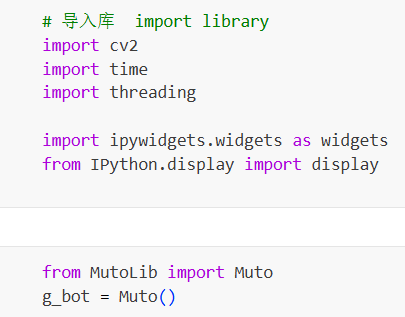
\includegraphics[width=0.49\linewidth]{pic/init.png}
        \end{center}
    \end{figure}
\end{frame}

\begin{frame}{代码实现-机器人控制}
    \begin{figure}[htpb]
        \begin{center}
            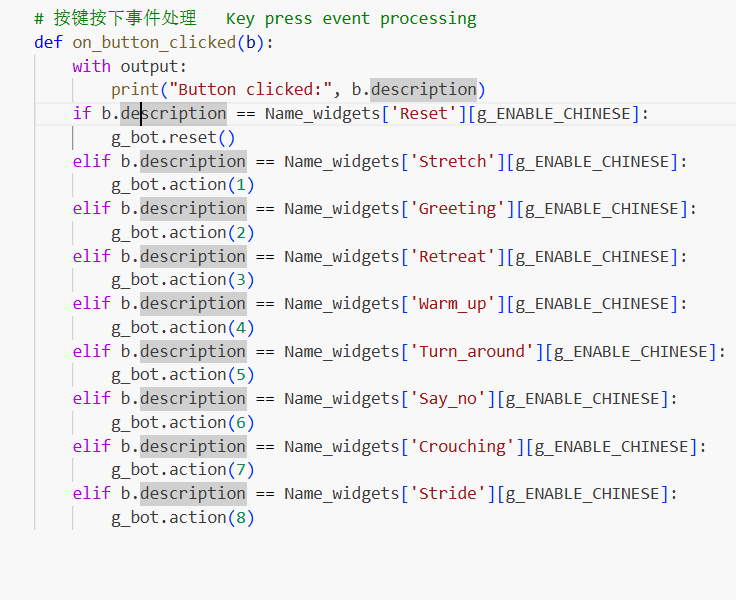
\includegraphics[width=0.49\linewidth]{pic/press1.png}
            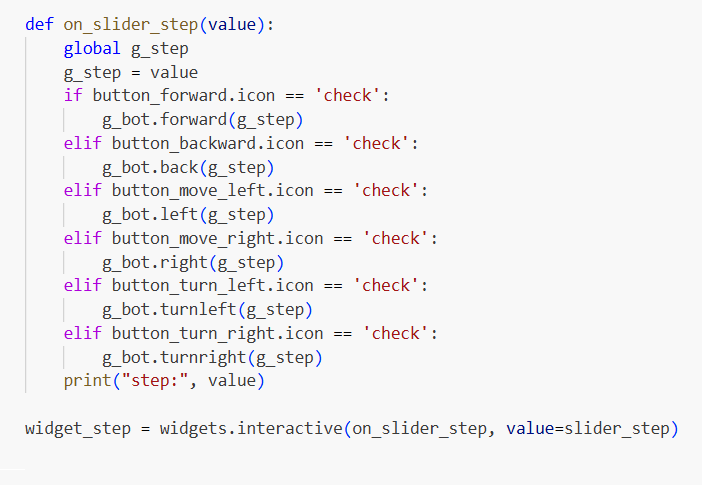
\includegraphics[width=0.49\linewidth]{pic/press2.png}
        \end{center}
    \end{figure}
\end{frame}

\begin{frame}{代码实现-机器人控制}
    \begin{figure}[htpb]
        \begin{center}
            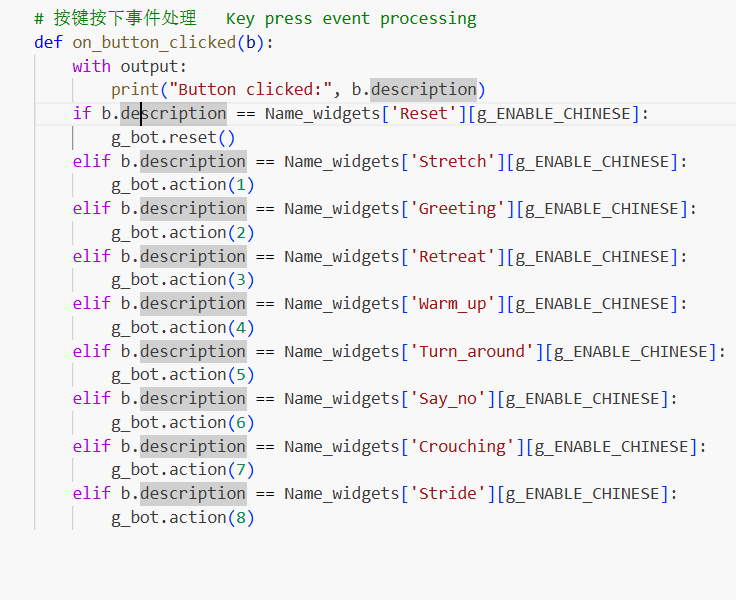
\includegraphics[width=0.49\linewidth]{pic/press1.png}
            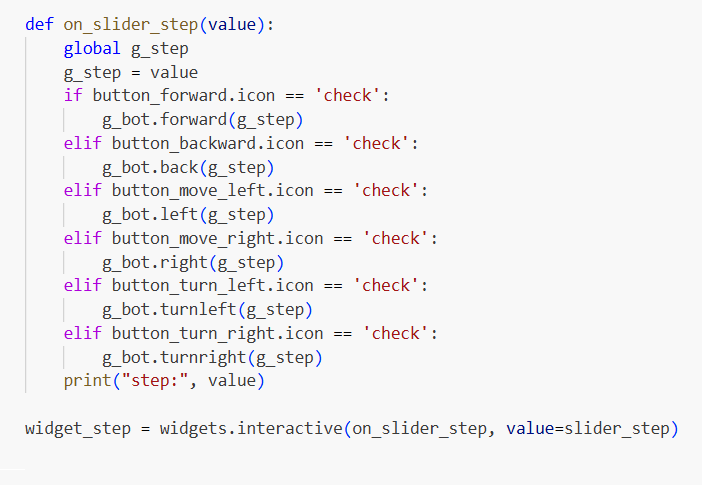
\includegraphics[width=0.49\linewidth]{pic/press2.png}
        \end{center}
    \end{figure}
\end{frame}

\begin{frame}{实现效果-表演动作}
    \begin{figure}[htpb]
        \begin{center}
            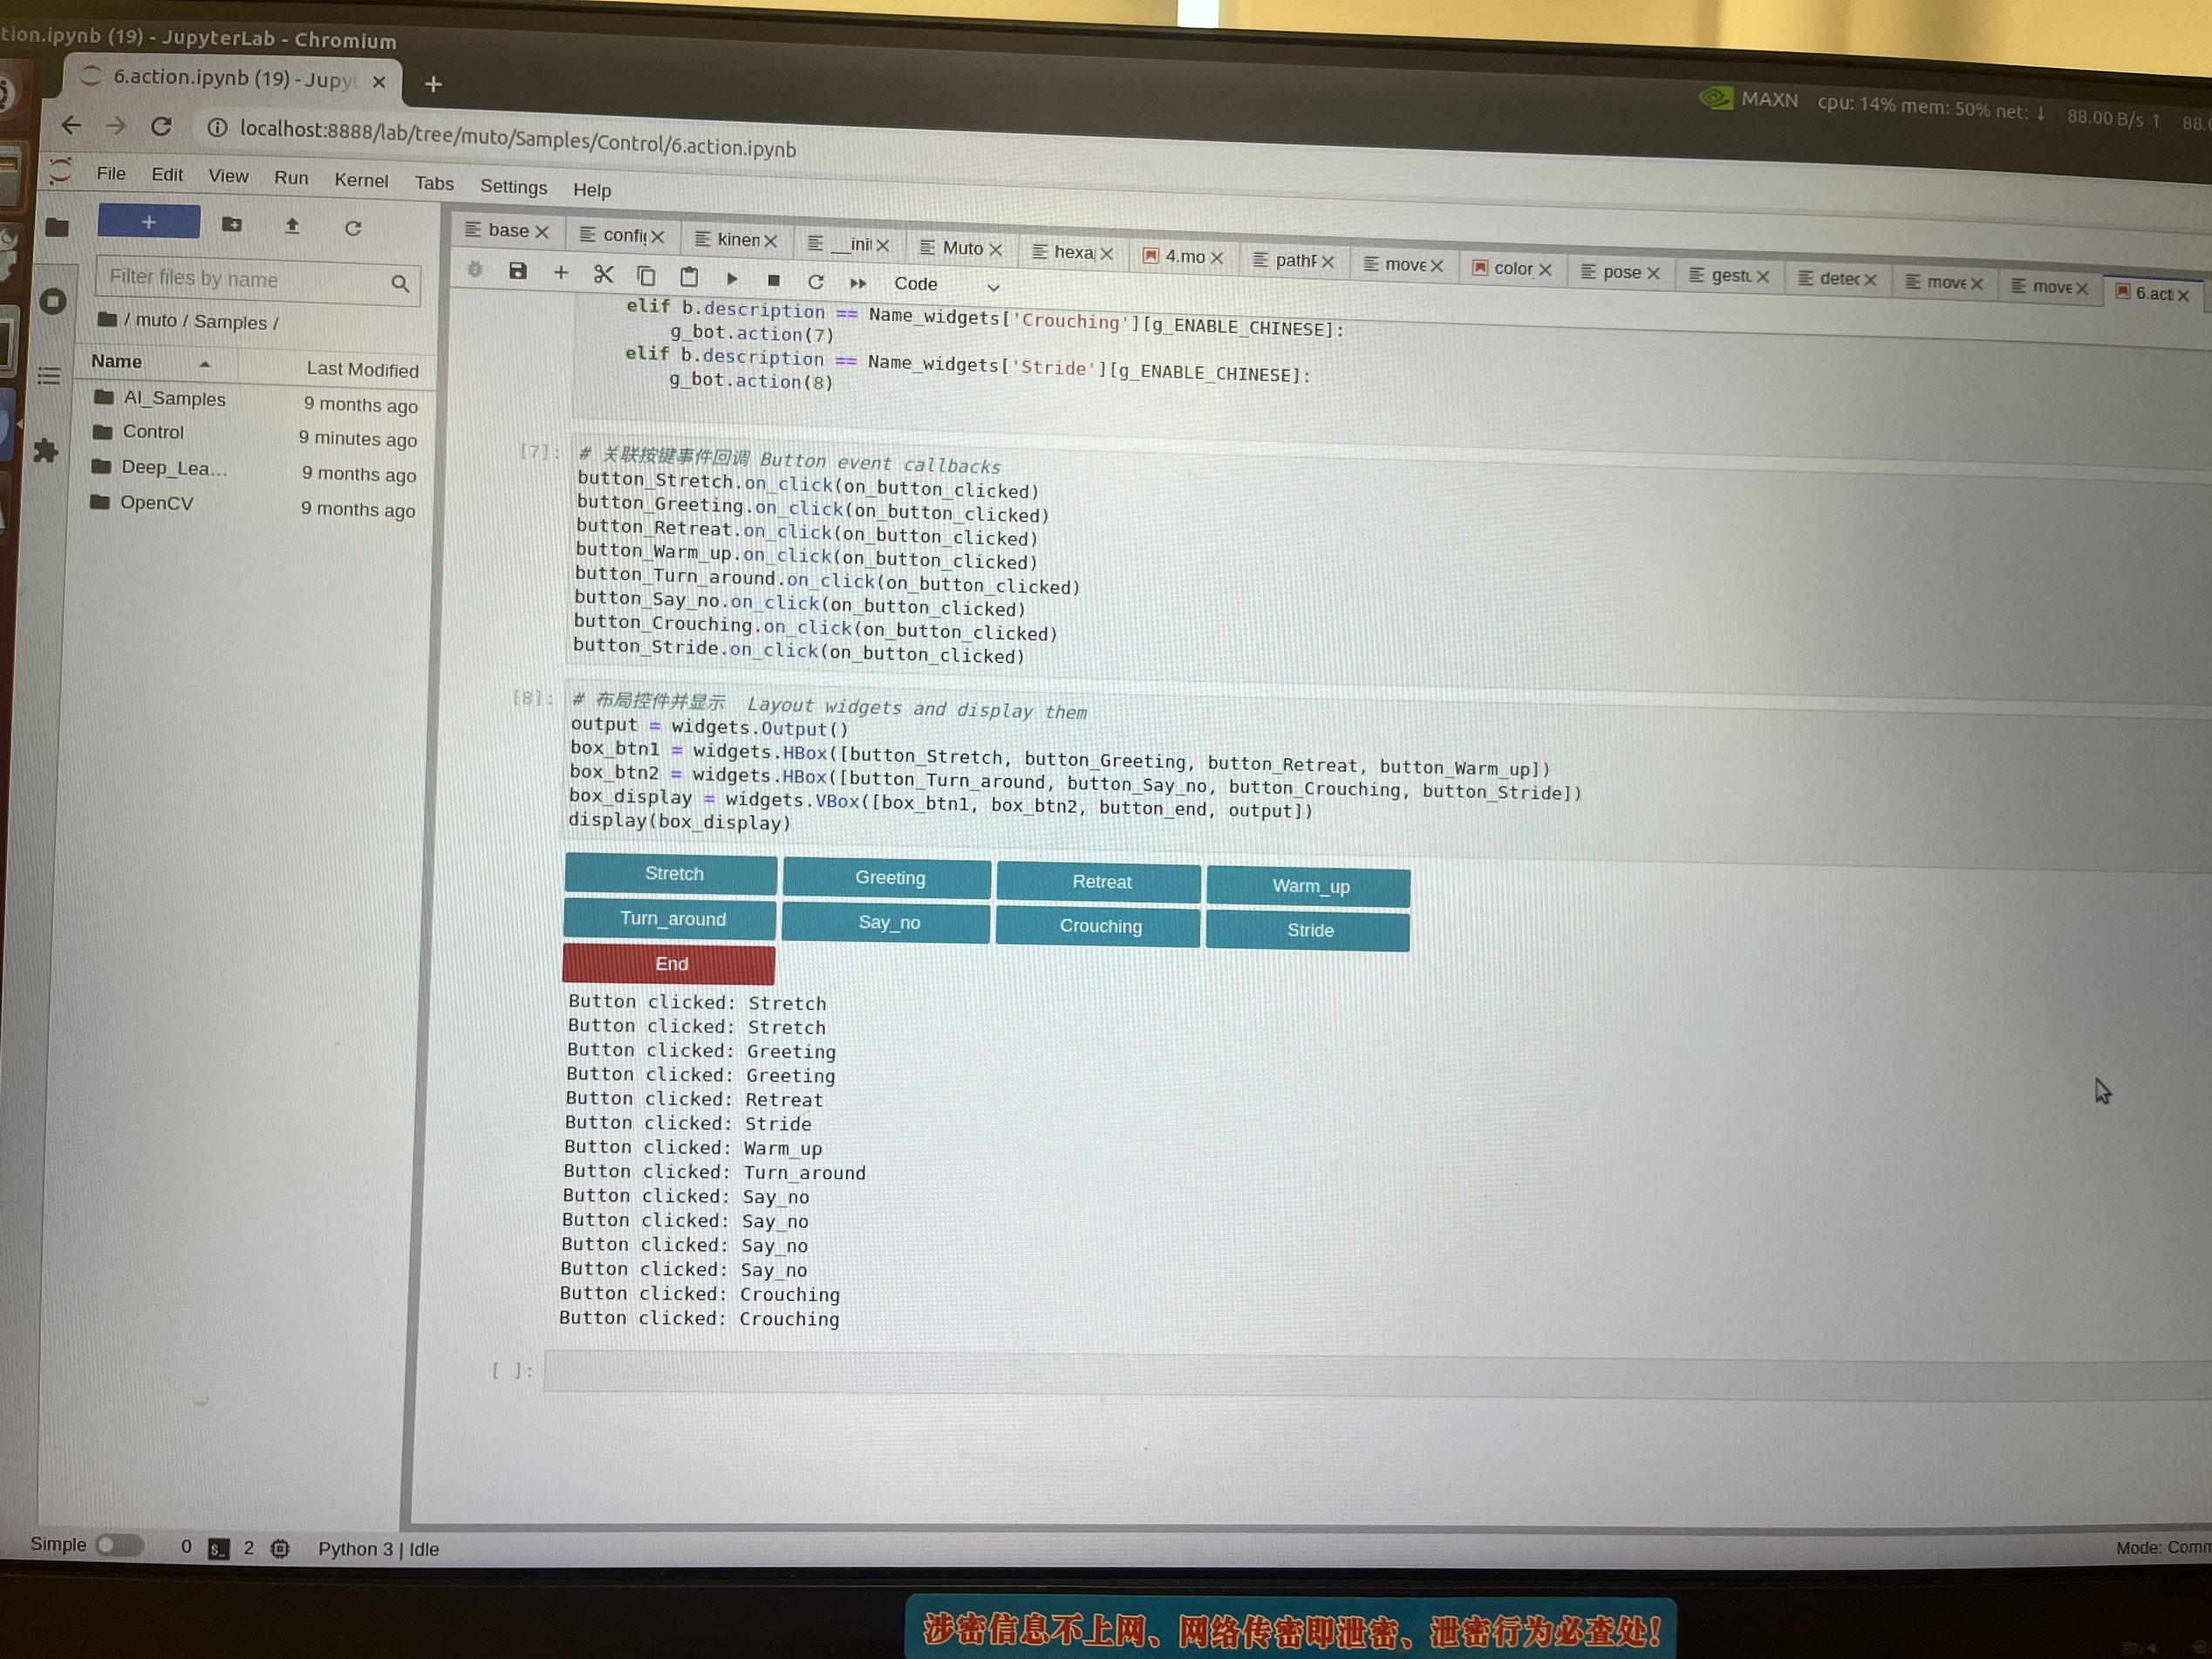
\includegraphics[width=0.8\linewidth]{pic/show1.jpg}
        \end{center}
    \end{figure}
\end{frame}

\begin{frame}{实现效果-基础控制}
    使用滑块空间来控制机器人的步长和速度。
    \begin{figure}[htpb]
        \begin{center}
            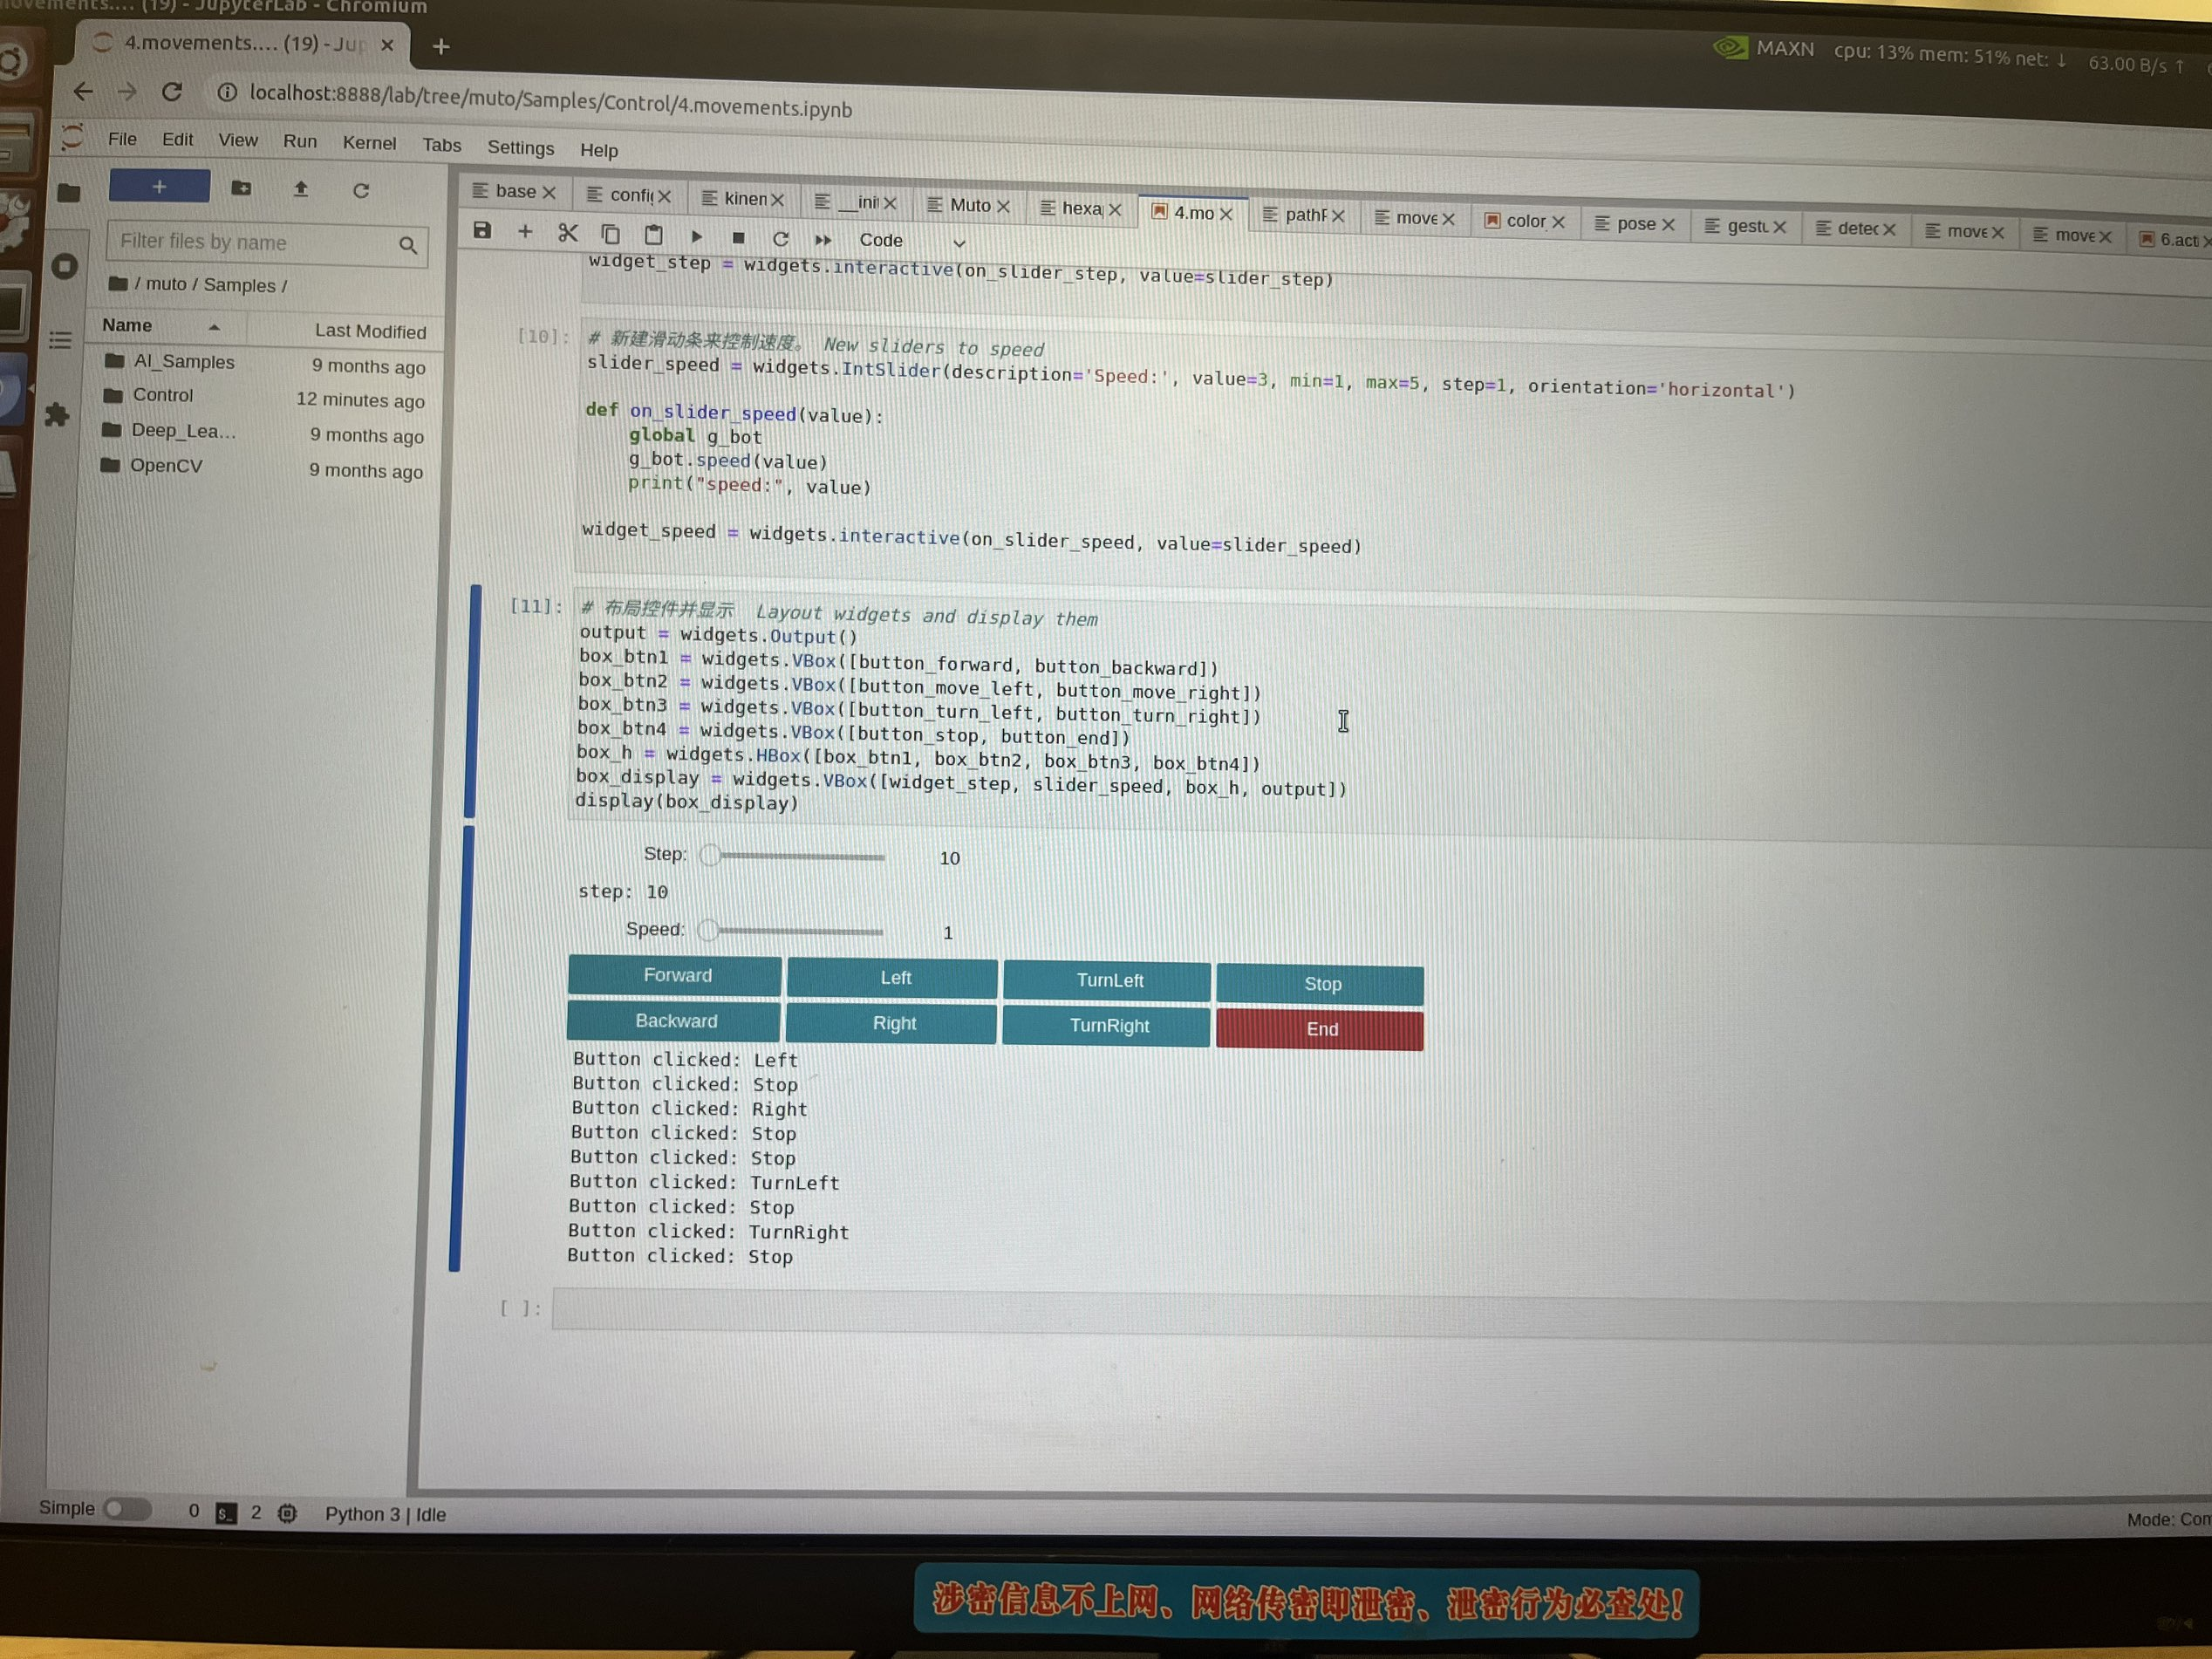
\includegraphics[width=0.8\linewidth]{pic/show2.jpg}
        \end{center}
    \end{figure}
\end{frame}

\section{机器人板载IMU模块研究}

\begin{frame}{IMU 模块介绍}
    \begin{figure}[htpb]
        \centering
        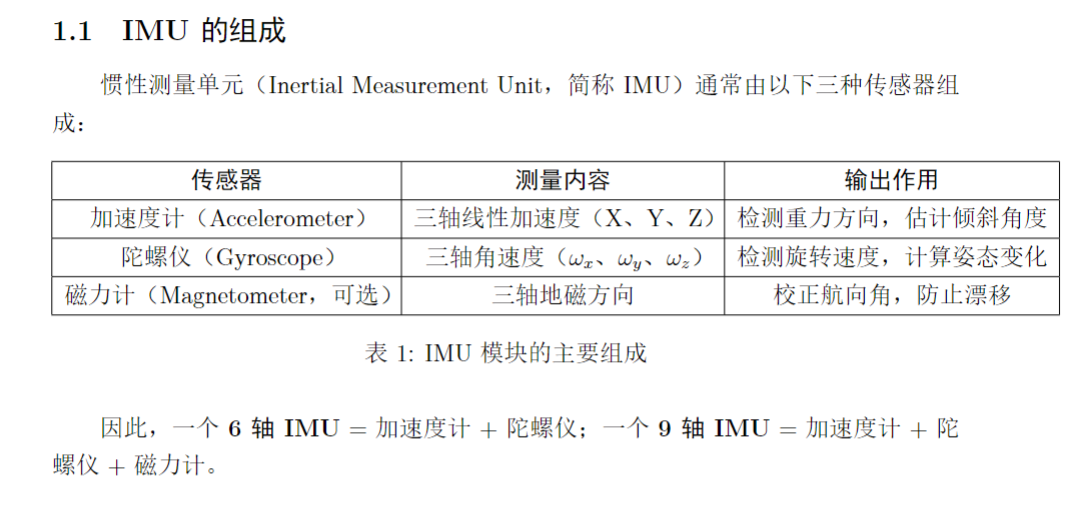
\includegraphics[width=1.0\linewidth]{pic/IMU.png}
    \end{figure}
\end{frame}

\begin{frame}{IMU 返回数据含义}
    \begin{table}[htpb]
        \centering
        \resizebox{0.9\linewidth}{!}{
        \begin{tabular}{|c|c|c|c|c|}
            \hline
            名称 & 中文名 & 含义 & 单位 & 典型范围 \\
            \hline
            roll & 横滚角 & 绕 X 轴旋转的角度，表示机器人左右倾斜程度 & \textdegree & -180\textdegree{} $\sim$ +180\textdegree{} \\
            \hline
            pitch & 俯仰角 & 绕 Y 轴旋转的角度，表示机器人前后倾斜程度 & \textdegree & -90\textdegree{} $\sim$ +90\textdegree{} \\
            \hline
            yaw & 航向角 & 绕 Z 轴旋转的角度，表示机器人朝向（转弯方向） & \textdegree & 0\textdegree{} $\sim$ 360\textdegree{} \\
            \hline
            temp & 温度 & IMU 模块内部温度 & \textcelsius & 一般 20 $\sim$ 40 \textcelsius \\
            \hline
        \end{tabular}
        }
    \end{table}
\end{frame}

\begin{frame}{上坡与俯仰角（pitch）的关系}
    当机器人上坡或下坡时，主要导致机身前后倾斜，因此与 \textbf{pitch（俯仰角）} 直接相关。
    \begin{itemize}
        \item 上坡时：前方抬高 $\Rightarrow$ pitch 增大（为正值）；
        \item 下坡时：前方降低 $\Rightarrow$ pitch 减小（为负值）。
    \end{itemize}

    \vspace{0.3cm}
    \textbf{示例：}
    \[
        \text{imu} = [0.54, 1.45, 51.77, 20]
    \]
    \begin{itemize}
        \item roll = 0.54\textdegree{}：机器人基本水平，无明显左右倾斜；
        \item pitch = 1.45\textdegree{}：机器人略微前倾，可能处于轻微上坡；
        \item yaw = 51.77\textdegree{}：机器人当前朝向；
        \item temp = 20\textcelsius：IMU 模块温度。
    \end{itemize}

    \begin{figure}[htpb]
        \centering
        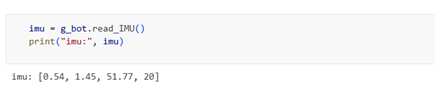
\includegraphics[width=0.65\linewidth]{pic/result.png}
    \end{figure}
\end{frame}

\begin{frame}{实验结果展示（一）}
    \textbf{结果：}
    \begin{figure}[htpb]
        \centering
        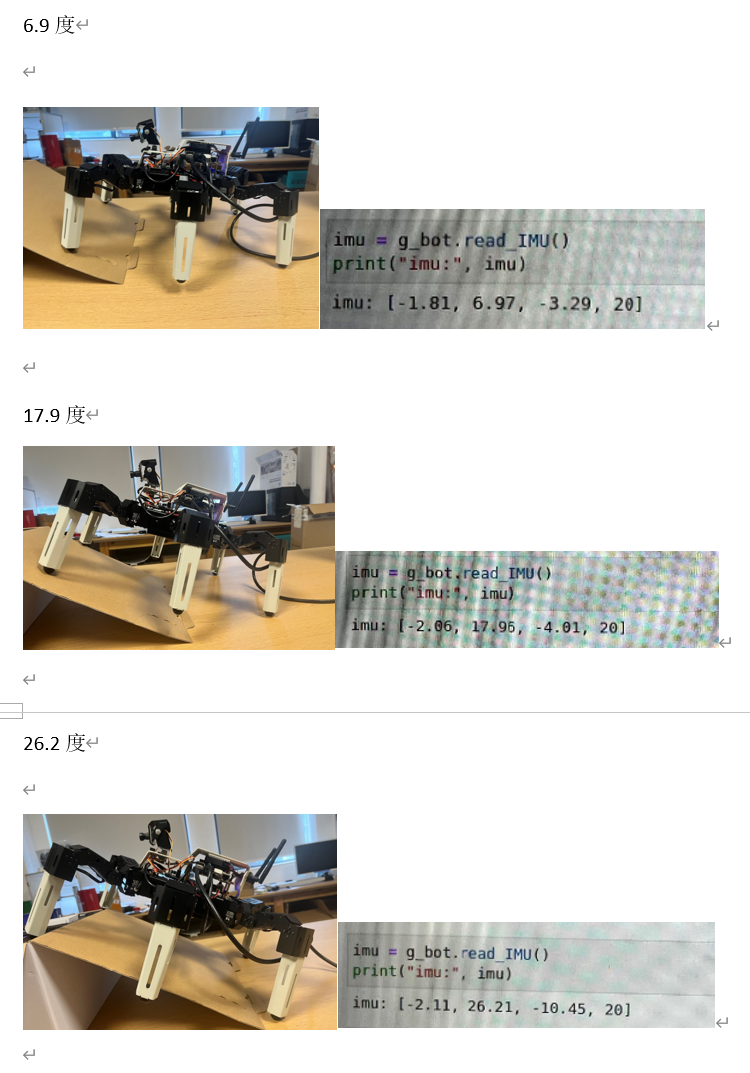
\includegraphics[width=0.4\linewidth]{pic/result-1.png}
    \end{figure}
\end{frame}

\begin{frame}{实验结果展示（二）}
    同样地，也可以通过 IMU 判断水平方向的倾斜：
    \begin{figure}[htpb]
        \centering
        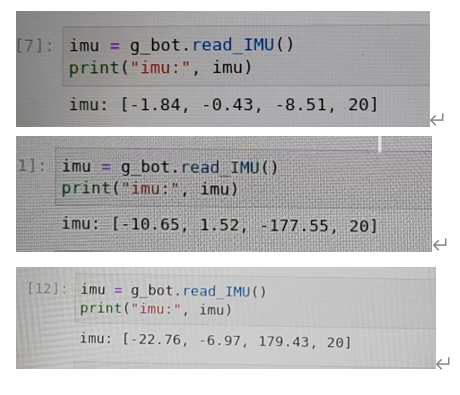
\includegraphics[width=0.7\linewidth]{pic/result-2.png}
    \end{figure}
\end{frame}

\section{避障功能实现}

\begin{frame}{代码分析}
    motor(servo\_id, angle, runtime=100)：控制机器人的十八个舵机转动。

    参数servo\_id表示要控制的舵机ID号，每个舵机ID号都不同，servo\_id的取值范围为[1, 18]，分别对应机器人上的18个总线舵机。

    参数angle表示要控制舵机运动到的角度，angle的取值范围为[-90,90]。

    参数runtime为可选参数，默认值为100，表示舵机运动的时间，在有效范围内，数值越小，转动速度越快。

\end{frame}

\begin{frame}{代码分析}
    Servo\_torque\_on（servo\_id=0）:打开舵机扭矩力。

    Servo\_torque\_off（servo\_id=0）:关闭舵机扭矩力。

    可选参数servo\_id表示要控制的舵机ID号，取值范围为[0, 18]，当servo\_id=0时，表示控制所有舵机扭矩力打开或关闭；当servo\_id=[1, 18]，表示控制对应ID号舵机扭矩力打开或者关闭。

    load\_leg（leg）:打开某一条腿上的三个舵机的扭矩力

    unload\_leg（leg）:关闭某一条腿上的三个舵机的扭矩力

    参数leg表示要控制的腿ID号，leg的取值范围为[1, 6]，分别表示机器人的六条腿。 
\end{frame}

\begin{frame}{控制逻辑}
    \begin{itemize}
        \item 机器人前行至障碍物前；机器人通过调用内置前进步态逐步接近障碍物，当前腿距离障碍物达到预设阈值时停止进入越障状态。
        \item 前腿跨越障碍物；前腿（Leg 1 与Leg 6）依次执行抬腿、跨越、落地动作。两条前腿均越过障碍物后，机器人前进，使中腿接近障碍物。
        \item 中腿跨越障碍物；中腿（Leg 2、Leg 5）动作逻辑与前腿一致，但为避免碰撞，需要更高的抬升角
度。中腿在跨越过程中承担机体主要支撑，因此其动作更加平缓，并结合IMU 姿态数
据进行微调。
        \item 后腿跨越障碍物。当前四条腿均处于障碍物前方时，机器人进入后腿跨越阶段。后腿（Leg 3、Leg
4）由于机体重心已前移，跨越动作更为顺畅，依旧遵循抬腿—跨越—落地流程。
    \end{itemize}
\end{frame}

\begin{frame}{模块化封装}
    \begin{figure}[htpb]
        \centering
        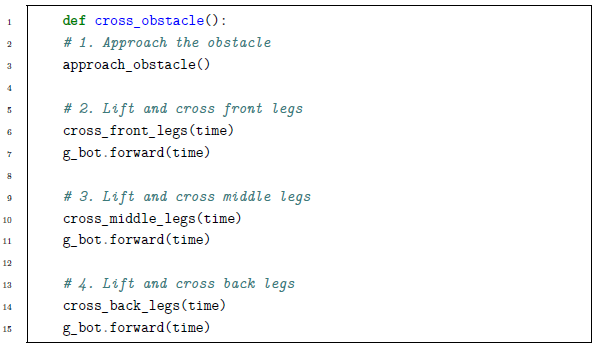
\includegraphics[width=0.8\linewidth]{pic/module3.png}
    \end{figure}
\end{frame}

\begin{frame}{实践效果}
    在六足机器人平台上，我们对所提出的避障功能进行了系统性的实验验证。该方
法适用于所有可近似为类长方体形状的障碍物，并在实验中验证了其在不同材料、尺
寸与环境条件下的稳定性。为了确保算法具有通用性，我们设定了如下适用条件：
\begin{itemize}
    \item 障碍物高度不得超过机器人腹部高度;
    \item 障碍物宽度不得超过机器人的标准步长;
\end{itemize}
实验中使用了泡沫块、木板箱体、塑料收纳箱、纸板箱等不同尺寸与材质的障碍
物。测试环境包含光滑实验室地面、轻微不平整的水泥地等多种场景。需要强调的是，
该方法不适用于坑洞、沟槽、落差、台阶、斜坡等凹陷或非凸形地形，此类场景由于
缺乏明确的可见几何外形，当前的行走机制无法支持有效位移。

\end{frame}

\section{总结和展望}

\begin{frame}{应用场景}
    在应用层面，该避障功能可用于多种实际场景，包括但不限于：
    \begin{itemize}
        \item 室内服务机器人任务（越过家具、储物箱等低矮障碍）;
        \item 仓储与物流环境（越过货物堆叠体、隔断板等矩形障碍）;
        \item 农业巡检与自然场地任务（越过低矮灌木、石块、农机具等简易障碍物）;
        \item 用于教学与科研的六足机器人平台，验证腿式移动的环境适应性.
    \end{itemize}
\end{frame}

\begin{frame}{人员分工}
    本项目的成员分工为：
    \begin{itemize}
        \item 曹洪珲负责前端UI 控件的调试实现与越障功能的实景测试；
        \item 黄育民负责后端机器人舵机控制交互的实现与设计越障动作。
        \item 谭诗弘负责相关文献资料的调研和驱动库阅读、PPT 和报告的撰写。
    \end{itemize}
\end{frame}

\begin{frame}
    \begin{center}
        {\Huge\calligra Thanks!}
    \end{center}
\end{frame}

\end{document}